\chapter{Literature Review}

% Approximately 5000 words  

%%%%%%%%%%%%%%%
% Basic Layout
%%%%%%%%%%%%%%%
% Introduction to Road Safety research in Ireland - What is the extent of the methods we research driver behaviour % 500
% Introduction to Decision Neuroscience % 2000
    % Typical Tasks
    % DDM
    % The speed accuracy trade off
    % The Kelly lab
    % EMG - How to use EMG for predictive modelling/prepratory signals
% Introduction to Traffic & Driver behaviour research
    % Try make this one 2000

%%%%%%%%%%%%%%%
% Introduction to Road Safety in Ireland
%%%%%%%%%%%%%%%
% Want this to be ~1000 words in sections
% The main focus is: How do we research driver behaviour
\section{Road Safety in Ireland - How Do We Research Driver Behaviour?}


\section{An introduction to decision neuroscience}
A common framework for these models is the drift diffusion model (DDM) developed by Ratcliff nearly 50 years ago \cite{ratcliffTheoryMemoryRetrieval1978}.


% Talk about the model in abstract
The DDM is a basic model of human decision making that can be used to understand decisions which correspond to the two alternative forced choice (2AFC) paradigm, where participants must make a binary decision quickly (within 2 seconds) with stimuli that are uncertain \cite{ratcliffDiffusionDecisionModel2008, myersPracticalIntroductionUsing2022}. The model allows an understanding of the neurological mechanisms which cause a decision to be made. In DDM the two alternatives of the 2AFC decision are modelled as the upper and lower boundary of the decision space. Within this space, following the onset of a stimulus, evidence accumulates noisily to one of the two boundaries with an average slope modelled by the drift rate $\nu$. Once one of the two boundaries have been crossed the decision will be recorded as having occurred at that time. This gives rise to the characteristic right skewed reaction time distributions seen in typical decision tasks \cite{ratcliffTheoryMemoryRetrieval1978}. A schematic of this process can be seen in \ref{fig:DDM plot}.
\begin{figure}
    \centering
    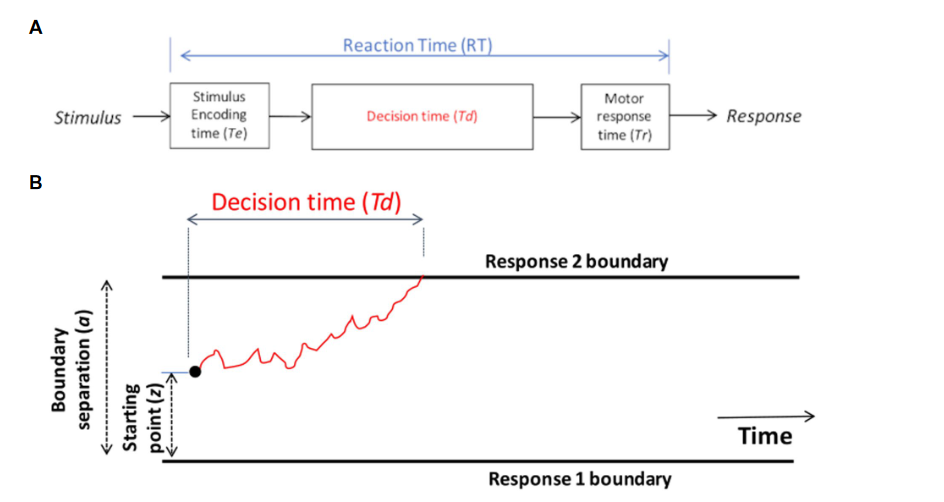
\includegraphics[width=0.75\linewidth]{figures/DDM.PNG}
    \caption{Schematic of the drift diffusion model (DDM). (A) Total reaction time to make a decision is composed of fixed stimulus encoding time $T_{e}$, decision time $T_{d}$ and motor response time $T_{r}$ (B) The noisy accumulation of data can be seen here from a starting point $z$ towards the two boundaries. The separation between the boundaries, seen here as $a$, can be manipulated with $z$ to bias the model towards one of the responses \cite{myersPracticalIntroductionUsing2022}}
    \label{fig:DDM plot}
\end{figure}

% random dot motion taske
This model has been studied in detail using simple decision tasks such as the random dot motion (RDM) task but has also been applied to more complicated tasks including the detection of military targets \cite{heitzNeuralMechanismsSpeedAccuracy2012}. The RDM task is one of the most common in use in the field and has been altered for study in a variety of ways to examine different factors. The basic structure of the task is the discrimination between coherent and incoherent motion; the dots begin by moving incoherently and at the onset of the simulus a certain subset of the dots begin moving coherently in a direction \cite{brittenAnalysisVisualMotion1992}. The participant must respond when they have identified the presence this stimulus. This task has been used to examine the effects of sleep deprivation, depression and, to help identify decision-related signals in the brain, among other applications \cite{ratcliffDiffusionModelOnechoice2011, kellyInternalExternalInfluences2013, whiteUsingDiffusionModels2010}. The task is useful in part because of the control it gives researchers over the difficulty of the task, forcing participants to make mistakes and giving a temporal distribution of both correct and incorrect reactions to fit models to.
% Another figure in here.
\begin{figure}
    \centering
    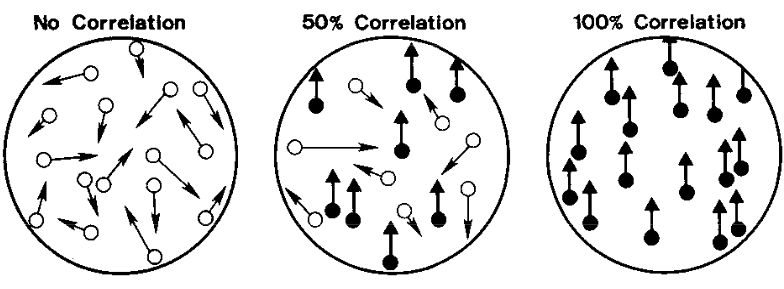
\includegraphics[width=0.75\linewidth]{figures/dots.PNG}
    \caption{A typical RDM task \cite{brittenAnalysisVisualMotion1992}}
    \label{fig:RDM}
\end{figure}


% Talk about why that can be applied to my situation
The models discussed in Geuzebroek et al are of particular note due to their focus on the decision making mechanisms that occur during a continuous monitoring task with intermittent detection of stimuli \cite{geuzebroekBalancingTrueFalse2023}. This is a similar context to that which is the focus of this thesis; a driver must continuously monitor the situation in front of them and respond to a series of intermittent encounters with cyclists. Of the variety of models examined the best fit to the model was found to be the criterion adjustment model, a schematic of which can be seen in \ref{fig:Anna}. In this model the evidence accumulation was referenced to a zero criterion point that could be adjusted among task difficulty contexts. How these difficulty contexts can be understood in the context of a driving task will be the subject of further discussion.
Having a model which has been built to fit to this format of decisions allows us to parametrise behavioural data as it is gathered from the experiment. This will then allow us to examine the influence of a series of factors on the decisions that are made by subjects.
\begin{figure}
    \centering
    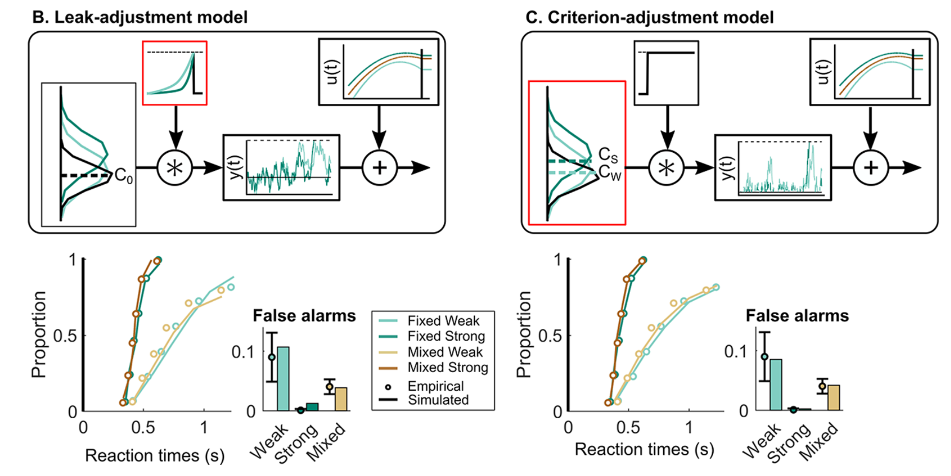
\includegraphics[width=0.75\linewidth]{figures/Anna.PNG}
    \caption{A figure from Geuzebroek et al comparing the fits of the B) leak-adjustment and C) criterion-adjustment models that were examined in the paper. While it is not clear which of the fits was better from this model what can be seen is that the models were successful in simulating data similar to the observed data \cite{geuzebroekBalancingTrueFalse2023}}
    \label{fig:Anna}
\end{figure}

% 'Metacognition'
% Gap acceptance and the follow up paper
% How has decision neuroscience

%% EMG Preparatory signals & confidence in decision making

% Can
